\documentclass[dvipdfmx,cjk]{beamer} 
%\documentclass[dvipdfm,cjk]{beamer} %% オプションは環境や利用するプログラムに
%\documentclass[dvips,cjk]{beamer}   %% よって変える

\AtBeginDvi{\special{pdf:tounicode 90ms-RKSJ-UCS2}} %% しおりが文字化けしないように
%\AtBeginDvi{\special{pdf:tounicode EUC-UCS2}}

%\setbeamertemplate{navigation symbols}{} %% 右下のアイコンを消す

\usetheme{CambridgeUS}         %% theme の選択
%\usetheme{Boadilla}           %% Beamer のディレクトリの中の
%\usetheme{Madrid}             %% beamerthemeCambridgeUS.sty を指定
%\usetheme{Antibes}            %% 色々と試してみるといいだろう
%\usetheme{Montpellier}        %% サンプルが beamer\doc に色々とある。
%\usetheme{Berkeley}
%\usetheme{Goettingen}
%\usetheme{Singapore}
%\usetheme{Szeged}

%\usecolortheme{rose}          %% colortheme を選ぶと色使いが変わる
%\usecolortheme{albatross}

%\useoutertheme{shadow}                 %% 箱に影をつける
%\usefonttheme{professionalfonts}       %% 数式の文字を通常の LaTeX と同じにする

%\setbeamercovered{transparent}         %% 消えている文字をうっすらと表示する


\setbeamertemplate{theorems}[numbered]  %% 定理に番号をつける
\newtheorem{thm}{Theorem}[section]
\newtheorem{proposition}[thm]{Proposition}
\theoremstyle{example}
\newtheorem{exam}[thm]{Example}
\newtheorem{remark}[thm]{Remark}
\newtheorem{question}[thm]{Question}
\newtheorem{prob}[thm]{Problem}





\begin{document}
\title[Beamer]{パーシステント・ホモロジーを利用した\\センサーデータの分析} 
\author[TUS]{黒木 裕鷹}            %% ここに書かれた情報は色々なところに使われるので
\institute[Tokyo University of Science.]{東京理科大学}   %% なるべく設定した方が良い
\date{May 11, 2018}

\begin{frame}                  %% \begin{frame}..\end{frame} で 1 枚のスライド
\titlepage                     %% タイトルページ
\end{frame}

\begin{frame}                  %% 目次 (必要なければ省略)
\tableofcontents
\end{frame}

\section{はじめに}             %% セクション名
\begin{frame}
\frametitle{はじめに}              %% フレームタイトル

\begin{itemize}
\setlength{\itemsep}{8mm}
\item 工場の生産ラインでは様々な産業用ロボットが用いられている
\item ロボットは効率的である反面,故障のリスクがつきまとう
\item 多くの現場ではメンテナンスを委託または経験則に基づくタイミングで行なっている
\end{itemize}
\end{frame}

\begin{frame}{ロボットのメンテナンス}
\centerline{効率的な生産ラインの実現にロボットのメンテナンスは不可欠}
\vspace{8mm}
\begin{itemize}
\setlength{\itemsep}{6mm}
\item メンテナンスのために生産ラインを止めることは望ましくない
\item 故障直前のデータを取得することが難しく,教師あり学習による分類は困難
\end{itemize}
\end{frame}

\begin{frame}{センサーデータ}
\begin{itemize}
\setlength{\itemsep}{8mm}
\item ロボットのモニタリングは振動や温度などのセンサーで行われる
\item ロボットのメカニズムによらない解析では,スペクトル解析や統計量による解析が一般的
\item 時系列クラスタリングが難しい話がしたいが,データの不備の話をしなくてはならない...
\end{itemize}
\end{frame}

\section{先行研究}
\begin{frame}
\begin{itemize}
\setlength{\itemsep}{8mm}
\item 異常検知の王道.ほとんどが正常と思われるデータが必要.データ不備の話をここでも・・・・・
\item スペクトルに関する話もする?ICAを行えない歯がゆさ
\end{itemize}
\end{frame}

\section{TDA}             %% 文字の色を変える
\begin{frame}{データの位相的特徴}
\begin{itemize}
\setlength{\itemsep}{8mm}
\item 近年,データの位相的特徴を見るTopological Data Analysis(TDA)が近年注目されている
\item Stochasticな手法では得られない新たな知見を獲得する狙い
\item 核となる方法はpersistent homologyやmapperなど
\end{itemize}
\end{frame}

\begin{frame}{目的}
\begin{alertblock}{課題}
\begin{itemize}
\item 不備があり,かつ明確に異常だと分からないセンサーデータから知見を得たい
\item 観測の同時性を考慮しないアプローチを考える
\end{itemize}
\end{alertblock}
\centerline{\Huge$\downarrow$}
\begin{exampleblock}{目的}
\begin{itemize}
\item TDAのメソッドを時系列データに適用する
\item 抽出した位相的特徴を元にした教師なし学習を提案する
\item データ・ドリブンなロボット管理を目指す.
\end{itemize}
\end{exampleblock}
\end{frame}

\section{手法}
\begin{frame}{persistent homology}
persistent homologyとは,ホモロジーの生起と消失を見るメソッドである
\vspace{5mm}
\begin{figure}[H]
\begin{center}
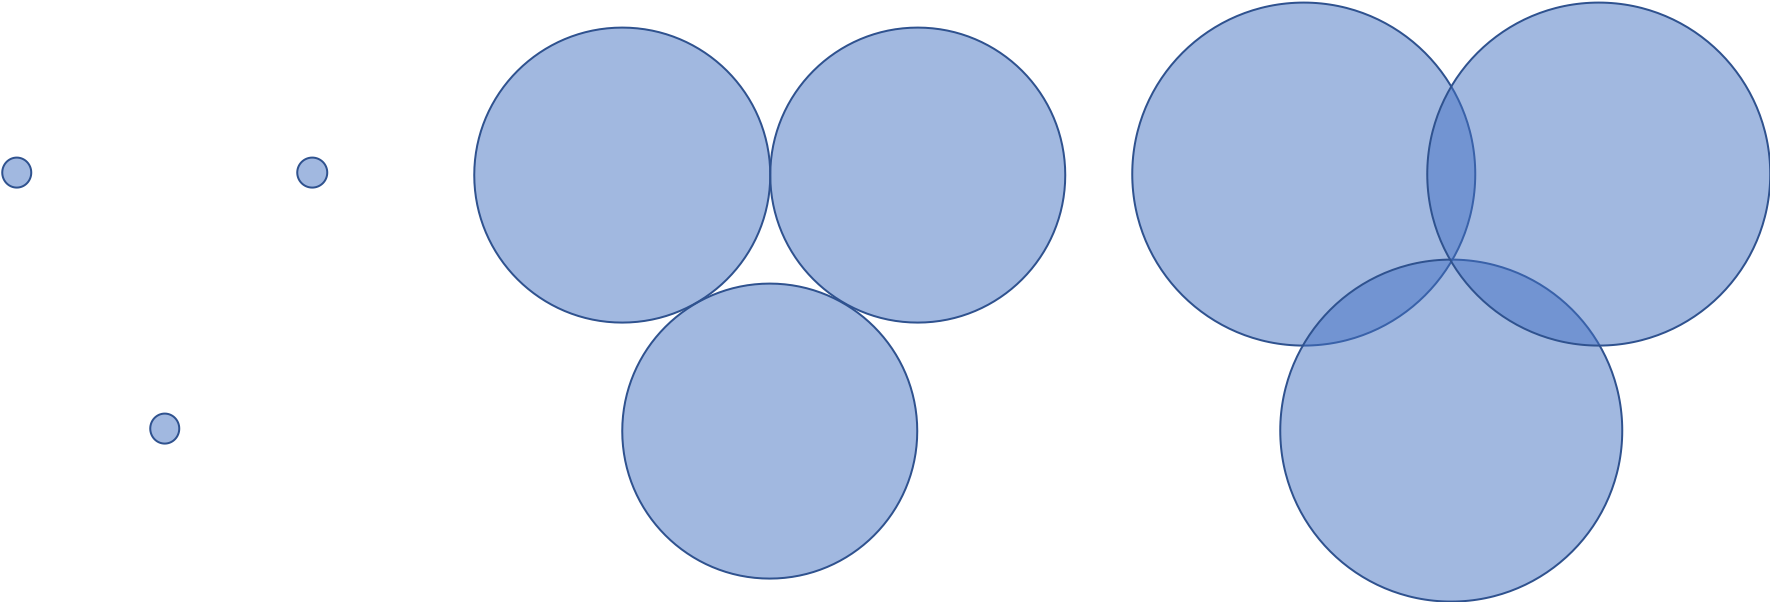
\includegraphics[width=100mm]{fig/persistent_homology.png}
\caption{1次persistent homologyの例}\label{fig:PH}
\end{center}
\end{figure}
\end{frame}


\begin{frame}{persistent diagram}
\begin{itemize}
\item persistent homologyの一意な表現
\item 横軸がホモロジーが生起する半径
\item 縦軸がホモロジーが消失する半径
\item 散布図であり,解釈し難い
\end{itemize}
\begin{figure}[H]
\begin{center}
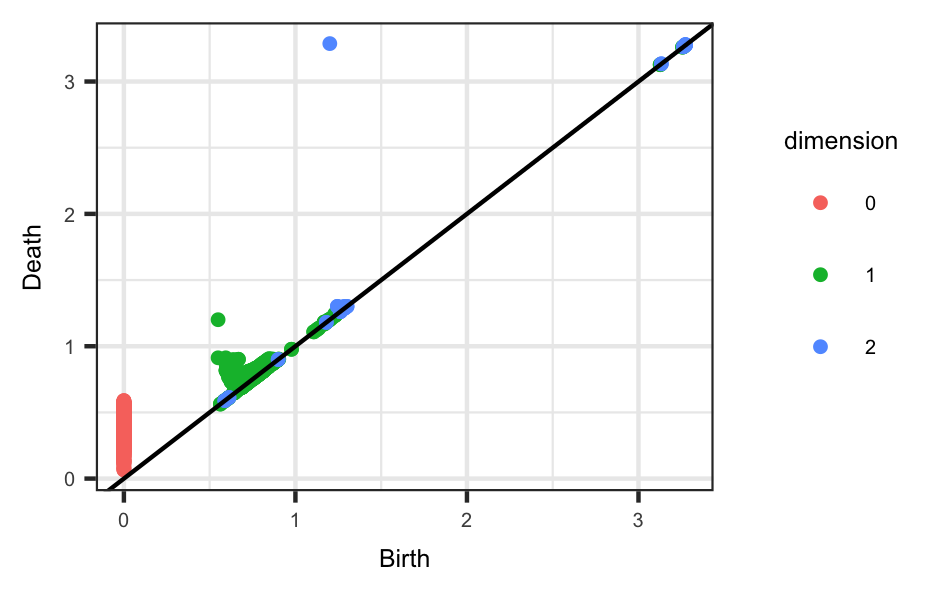
\includegraphics[width=90mm]{fig/persistent_diagram.png}
\caption{1次persistent diagramの例}\label{fig:PD}
\end{center}
\end{figure}
\end{frame}

\begin{frame}{persistent diagramの要約}
\begin{itemize}
\item 様々なpersistent diagramの要約が提案されてきた
\item maximum persistent
\end{itemize}
\end{frame}

\begin{frame}{Betti sequence}
\begin{itemize}
\item 何個のホモロジーが存在しているかの,半径の時系列.
\item 以下で定義される
\end{itemize}
\end{frame}

\section{データ解析}
\begin{frame}{使用データ}
\begin{itemize}
\item 自動車メーカーMの産業用ロボットアーム
\item 振動データ
\item ロボットアーム15種
\item 減速機交換前後
\item 各10回計測
\end{itemize}
\end{frame}

\begin{frame}{多次元への埋め込み}
単位1の遅れ時間座標により7次元に埋め込み,PCAで3次元に次元圧縮
\end{frame}

\begin{frame}

\end{frame}


\section{考察・今後の課題}

\begin{frame}{今後の課題}

\end{frame}

\end{document}